\documentclass[10pt,a4paper]{article}
\usepackage[utf8]{inputenc}
\usepackage{amsmath}
\usepackage{amsfonts}
\usepackage{float}
\usepackage{amssymb}
\usepackage{graphicx}
\author{Zena Poudel}
\title{Huffman Coding}

\begin{document}
	\maketitle
	\section{Intro to Communication System}
	\begin{figure}[htp]
		\centering
		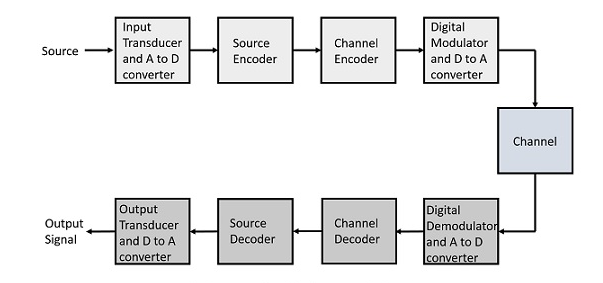
\includegraphics[width=10cm]{Image 1}
		\caption{Digital Communication System}
		\label{fig:Image 1}
	\end{figure}
	Communication system is system that transfer information from it’s source to destination some distance away. Information indicates higher dimension of message. Information are obtained from messages. Some message have higher information and some have lower. Higher the probability of any event in message to occur the lower that message will have information. and vice versa. Information is inversely proportional to probability. 
	
	Output from any source can be digital(Computer o/p, text) or analog (speech, video) signal. Although analog signal are easier to process but due to undesirable signal disturbances, data loss, subjection toward noise and other issues, in modern communication system, analog signal are also digitized. Digital message consist of sequence of binary bits. 
	\section{Coding and modulation}
	Signal-processing by varying one or more of the amplitude, frequency or phase of waveform by imposing an input signal on a carrier wave is known as modulation. Different types of modulation- 
	\newline
	Analog modulation - Amplitude Modulation (AM), Frequency Modulation (FM), Phase Modulation (PM) 
	\newline 
	Digital modulation - Amplitude Shift Keying, Frequency Shift Keying, Phase Shift Keying, e.t.c
	\newline
	Pulse Digital Modulation - Pulse Amplitude Modulation (PAM), Pulse Time Modulation (PTM), Pulse Position Modulation, Pulse Code Modulation (PCM) 
	\newline

	Whereas symbol processing  by converting digital messages into new sequence of symbols is coding. 
	
	Consider digital source having $ M >> 2 $ symbols. Uncoded transmission of messages require $ M $ different waveforms, one for each symbol. Alternatively each symbol could be represented by binary codeword consisting of $ k $ binary digits. $2^k$ possible codewords made up of k binary digits, we need $k>= log_2 M /$ digits codeword to encode M source symbols. For example we have message "ahfkjebf" which requires 8 different waveform but converting into binary symbol with 3 digits $ [ k = log_2 8] = 3$. 
	
	Coding and representing any data into binary digits have following two general advantage:- 
	\begin{enumerate}
		\item 	Less complicated hardware is required (just two different waveform) 
		\item  Noise have less effect in binary signal.  
	\end{enumerate}

	Basically there are 4 main reason for coding. Different types of encoding are done as per requirement. We perform source encoding in order to reduce the amount of data to be transmitted. Data compression or source encoding focuses on reduction of size of data but while doing so, the data can also be encrypted but the main focus remain same. 
	\newline
	\newline
	While transmitting messages from source to destination through channels, different noises and distortions can be added in channels which leads to the addition of errors in data, to reduce error (which cannot be completely eliminated) we perform channel encoding or error correction encoding. 
	\newline
	\newline
	Encryption is done by converting messages into secret code in order to hide true meaning of data. 
	
	\begin{enumerate}
		\item Adapt to electrical or accidental characteristics of the channel   
		\item Reduce the amount of data to be transmitted (Source Coding )
		\item Control errors (Error Coding or Channel encoding)
		\item Conceal and hide data (Cryptography)
	\end{enumerate}
	 
	 Source coding is the process of encrypting the information such that unnecessary data are removed which leads to effective transmission by 
	 adjusting bandwidth and 
	 eliminating data redundancy.
	 Here the main motto of source coding is to compress the size of data.
	 \newline
	 One example how we can adjust bandwidth is:- 
	 \newline
	 Information is inversely proportional to probability of any event to occur. If source s1 have message whose probability of occurrence is too high then it is sure to be occurred and no new and important information is carried by source, here information carried by this source is really small. So  small number of bits are provided for this message and if source s2 have message whose probability of occurrence is too low then more number of bits are provided. Doing so , we can adjust the bandwidth for different sources.
	 
	 \subsection{Fixed length and variable length coding}
	 
	 Fixed length coding is the coding method where code generated for every symbol will be having fixed length or equal no. of bits. For example
	 if we have 5 symbols;- a,b,c,d,e we may have 3 digit binary source-code for each of them  as follows:-
	 \newline
	 a - 000\newline
	 b - 001\newline
	 c - 010\newline
	 d - 011\newline
	 e - 100
     
     Variable length coding is coding method where various symbols of any message will be represented with different no. of bits.  Example: Huffman coding, Shannon Fano coding. For example if we have 5 symbols;- a,b,c,d,e we may have different digit binary source-code for each of them  as follows:-
     \newline
     a - 0\newline
     b - 1\newline
     c - 01\newline
     d - 11\newline
     e - 00\newline
     
     Let source s1 have message "bad". If we encode this message with above fixed length code and variable length code, then we have following encoded value-
     \begin{enumerate}
     	\item In fixed length codig:- 
     	bad - 0010000111
     	\item In Variable length coding:-
     	bad - 1011
     \end{enumerate}
     From above codewords, we can see, variable length coding definitely requires less amount of bits. Now while decoding- 
     \begin{enumerate}
     	\item In fixed length codig:- We know each symbol have fixed length code, in this case each symbol have 3 binary digits. So we go from left to right and assign symbol for each after checking in table. 
     	0010000111 \newline
     	001- b \newline
     	000 - a \newline
     	111 - d \newline
     	0010000111 - bad \newline
     	\item In Variable length coding:-
     	1011\newline 
     	here, when we try to decode the code, \newline  
     	1011 - 
     	1- b
     	0- a 
     	1- b 
     	1- b  
     	\newline or
     	1- b
     	0- a 
     	11- d  \newline
     	It is not possible to decode uniquely.     	
     \end{enumerate}
 
 To solve this, prefix free code was introduced. 
 \subsection*{Prefix free code}
 In prefix code, no variable length code word is a prefix of another. Following codes are an examples pf prefix free code. 
 \newline
 a - 00\newline
 b - 01\newline
 c - 10\newline
 d - 110\newline
 e - 111\newline
 Now, encoding "bad" will have following codeword:- \newline
 0100110. And decoding 0100110 gives "bad".
 
 \subsection{Lossless and lossy coding}
 Lossless:- Data can be decoded to form exactly the same bits. Better for text, code. example:- Huffman coding. \newline
 Lossy:- Some of the original data is removed. After the message is decoded it is not as same as original. coding algorithms that are characterized by an irreversible loss of information. Image, video, audio follows lossy compression. 
\section{Greedy algorithm paradigm }
\begin{enumerate}
	\item  Builds up a solution piece by piece.
	\item Next choice will be most obvious and immediate benefit.
\end{enumerate} 

It makes the choice that seems to be best at the moment.

\section{Huffman coding}
\begin{enumerate}
	\item  Variable length encoding (Prefix free code)
	\item Lossless data compression method
	\item Most probable elements are coded with less or few bits and least probable coded with greater no. of bits. 
	\item Follows greedy algorithm paradigm. 
	\item Optimum Prefix source coding with  O(N.log N) complexity.
	\item Generally include 2 steps:-
	\begin{itemize}
		\item Build Huffman tree 
		\item Traverse Huffman tree and assign codes.
	\end{itemize}
\end{enumerate} 
\section*{Steps in building Huffman tree}
While building huffman tree, we choose two symbols with minimum probability. For this, we use minimum heap. Following steps are followed in building Huffman tree:-   
\begin{enumerate}
	\item Select the two letters ai and aj with the smallest probabilities and create a parent node for the nodes that represent these two letters in the binary code tree. 
	\item Replace the letters ai and aj by a new letter with an associated probability of p(ai) + p(aj ). 
	\item If more than one letter remains, repeat the previous steps. 
	\item Convert the binary code tree into a prefix code
\end{enumerate}
Let us assume that there are "n" number of symbols, $s_1$, $s_2$, ..... , $s_n$ with probabilities $p_1$, $p_2$,...., $p_n$. We build min heap tree w.r.t frequencies. Then delete the node and fix the heap. And merge 2 minimum probabilities. Complexity of this step depends on the height of the tree i.e. 0(logn). This step is done for n times. Here total complexity is O(n. logn). And 2 minimum nodes are merged for n times, this implies complexity for merging is O(n). 
Hence, Complexity for building huffman tree is O(n. logn).
\section*{Example of huffman coding}

\begin{center}
\begin{tabular}{ c c }
		source & probabilities\\
		s1 & 0.1  \\ 
		s2 & 0.3 \\  
		s3 & 0.2  \\ 
		s4 & 0.1  \\
		s5 & 0.3 \\ 
\end{tabular}
\end{center}

From above table, s1and s4 have least probabilities. Add probabilities of s1 and s4 and store in s1s4 whose probability will be 0.2. Now s1s4 and s3 have least probabilities. Add s1s4 and s3 and store in s1s4s3 whose probability will be 0.4. Now s2 and s5 have least probabilities. Add s2 and s5 and store in s2s5 whose probabilities will be 0.6. Now add s1s4s3 and s2s5 and store in s1s4s3s2s5 whose probability will be 1. 
\begin{figure}[H]
    	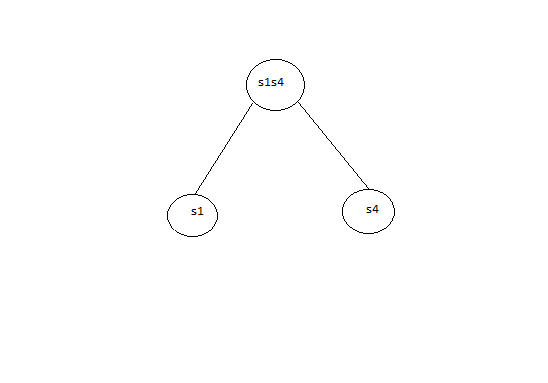
\includegraphics[scale=0.9]{eg1}
    	\caption{1st step}
    	\label{huffman1}
\end{figure}
\hfill
\begin{figure}[H]
	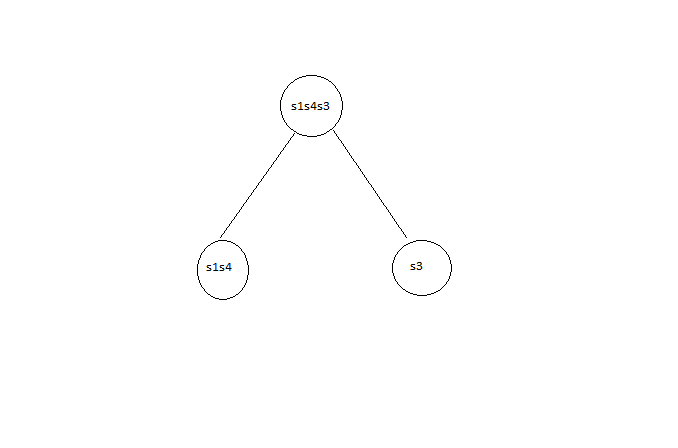
\includegraphics[scale=0.9]{eg2}
	\caption{2nd step}
	\label{huffman2}
\end{figure}
\hfill
\begin{figure}[H]
	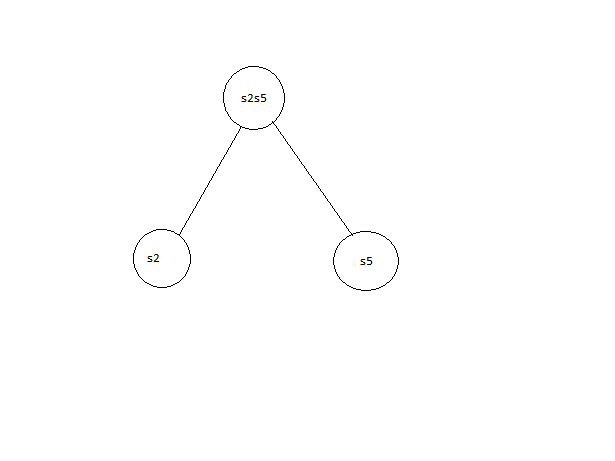
\includegraphics[scale=0.9]{eg3}
	\caption{3rd step}
	\label{huffman3}
\end{figure}
\hfill
\begin{figure}[H]
	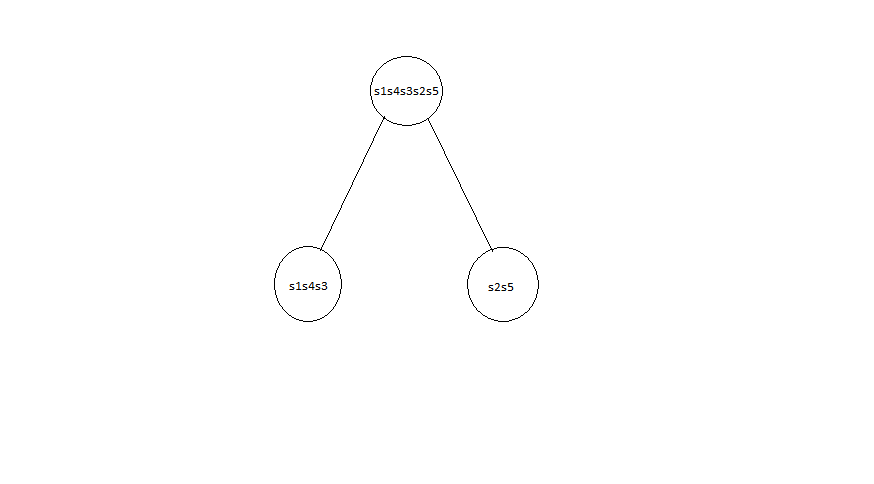
\includegraphics[scale=0.9]{eg4}
	\caption{4th step} 
	\label{huffman4}
\end{figure}
\hfill
Now combine tree keeping least probabilities node in left and vice versa. Then assign 0 to left and 1 for right.
\begin{figure}[H]
	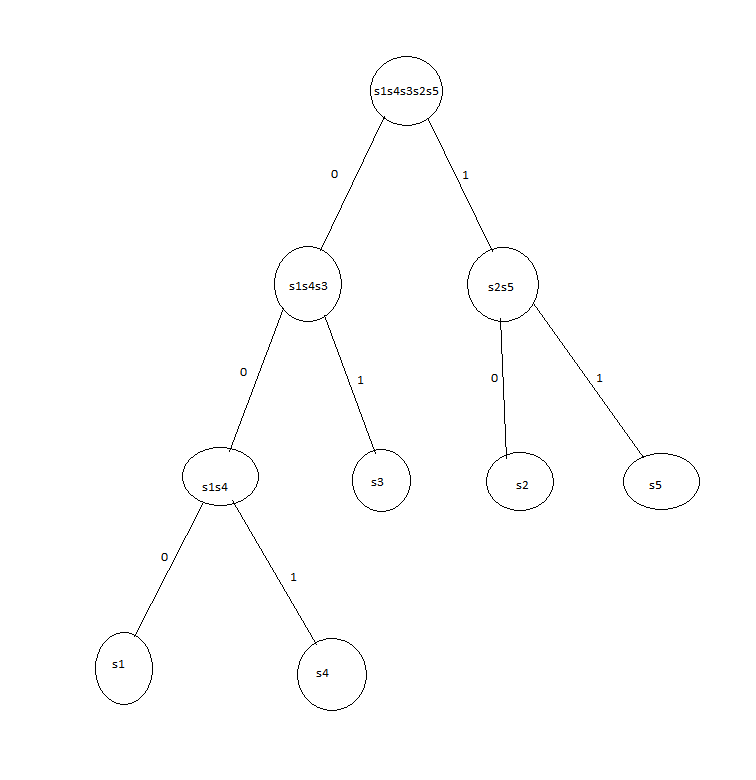
\includegraphics[scale=0.9]{final}
	\caption{Huffman Tree} 
	\label{huffman}
\end{figure}
\hfill
Now, let us complete above table providing code for each symbol.
\begin{center}
\begin{tabular}{ c c c }
	source & probabilities & code\\
	s1 & 0.1 & 000 \\ 
	s2 & 0.3 & 10 \\  
	s3 & 0.2 & 01\\ 
	s4 & 0.1 & 001\\
	s5 & 0.3 & 11\\ 
\end{tabular}
\end{center}
from above table, we have seen, symbol with high probability are coded with less bits and least probability have higher no. of bits. As information carried by symbol with higher probability is less and vice versa.
\section{Optimal Prefix code}
\begin{enumerate}
	\item  Given any two letters $a_j$ and $a_k$, if $ P(a_j) >= P(a_k) $ , then $ l_j <= l_k $, where $l_j$ is the length of the codeword $a_j$.  
	\item The two least probable letters have codewords with the same maximum length $l_m$. 
	\item In the tree corresponding to the optimum code, there must be two branches stemming from each intermediate node.  
	\item Suppose we change an intermediate node into a leaf node by combining all the leaves descending from it into a composite word of a reduced alphabet. Then if the original tree was optimal for the original alphabet, the reduced tree is optimal for the reduced alphabet. 

\end{enumerate}
Let us see if above example of huffman coding satisfies all condition of optimality or not. 
\begin{enumerate}
	\item  Comparing length of codeword for s1 and s2, probability of s2 is greater than s1, and length of codeword for s2 is shorter than s1.
	\item s1 and s4 are two symbols with least probability and both have codewords of 3 bit lengths, which is maximum length. 
	\item Intermediate nodes in any tree represents all node except leaf node, so if we take intermediate node (s1s4s3), we can see we have two  branches, 
	\item Let s1 and s4  is added and s1s4 is leaf node now, then we can see new three with leaf node s1s4, s3 , s2 and s5 is optimal. 
\end{enumerate}
Huffman coding satisfies all 4 condition.\\
\textbf{All Huffman codes are optimal prefix code but all optimal prefix codes are not Huffman codes. There can be other prefix codes which will be optimal.}
\section{Information, Average code length, Entropy and code efficency}
\subsection*{Information}
Information was not well defined  before Shannon's Information theory. But after Shannon published information theory, information is well- defined and measurable. If an outcome of any event is more improbable, then it will have more information and vice versa. Hence, information of any event is defined or measured in terms of probabilities. Messages and symbols are denoted in binary digits, so logarithms to the base 2 of inverse of the probability of that event determines information. Shannon's Information can be defined by following equation:- \\
\\
\\
\begin{equation}
 I = \log _{2} {\frac{1}{P}}
\end{equation}
where P is probability of occurance of symbol.
\subsection*{Entropy}
Entropy is measure of uncertainity or randomness. Hence it is one of the way to measure Information. The Shannon entropy of a distribution is the expected amount of information in an event drawn from that distribution. Simply,  Information entropy can be explained as an average of information, given by following equation:- \\
\begin{equation}
 H = \sum_{i=1}^{n} p_i log_{2}{\frac{1}{P}}
\end{equation}
where $P_i$ denotes $p_1, p_2,...., p_n$ are probabilities of occurance of symbols $s_1, s_2, ----,s_ n . $
\subsection*{Average code length}
Average code length can be defined as average number/length of  bits required to encode symbols. Average code length is given by following equation:- 
\begin{equation}
L = \sum_{i=1}^{n} p_i l_i 
\end{equation}
where $ P_i $ denotes $ p_1, p_2,...., p_n$ are probabilities of occurance of symbols $s_1, s_2, ----, s_n$ and $l_i$ denotes $ l_1, l_2 , ..., l_n$ are length of codewords for symbols $s_1, s_2, ....., s_n. $ \\
\subsection*{Code efficency}
Efficency is the measure of how well coding method encodes messages. It can be defined by following equation:- 
\begin{equation}
efficency (\eta ) =\frac {H}{L}
\end{equation}
\textbf{Entropy is a lower bound on average code length and entropy + 1 is upper bound on average code length for huffman code}\\
\\
$ H\leq L \leq H+1 $ \\
\\
\textbf{In our previous example, we can calculate efficency as:-} \\
\\
We know form eqn 2,\\
\\
$ H = \sum_{i=1}^{n} p_i log_{2} {\frac{1}{P}}$\\
\\
$ H =  0.1 * log_{2} {\frac{1}{0.1}} +  0.3 * log_{2}  {\frac{1}{0.3}} + 0.2 * log_{2}  {\frac{1}{0.2}} + 0.1 * log_{2}{  \frac{1}{0.1}} +  0.3 * log_{2}  {\frac{1}{0.3}}$ \\
\\
$ H = 2.1709$ \\
\\
We know form eqn 3, \\
\\
$L = \sum_{i=1}^{n} p_i l_i$ \\
\\
$ L =  0.1 * 3 +  0.3 * 2 + 0.2 * 2 + 0.1 * 3 +  0.3 * 2$ \\
\\
$ L = 2.2$\\
\\
Hence, from eqn 4, we know that, \\
\\
$ efficency (\eta ) =\frac {H}{L} $ \\
\\
$ efficency (\eta ) =\frac {2.1709}{2.2} $ \\
\\
$ efficency (\eta ) =0.9868 $ \\
\\
Here, efficency of huffman code is 98.68 $ \% $.
\\
\\
\textbf{In above example let us analyse upper and lower bound,} \\
\textbf{Lower bound :-} \\
$H \leq L$ \\
$2.1709 < 2.2 $ \\
$ True $\\
\\
\textbf{Upper bound :-} \\
$L \leq H+1$ \\
$2.2 < 3.1709 $ \\
$ True $\\
\section{Adaptive huffman coding}
In traditional or Conditional huffman coding that we explained, We previously have to know probability of symbol. That is we have to know which data we are going to encode before encoding, which is limitation of huffman coding. When the probability of symbols in
the information source is unknown, we have to calculate frequencies of occurance. This requires double pass of messages. Due to this reason, adaptive huffman coding was developed. \\
Steps in adaptive huffman coding:- \\
  
\begin{enumerate}
	\item  update tree.  
	\item encode.  
	\item decode
\end{enumerate}
Adaptive huffman coding :-
\begin{enumerate}
	\item Brute Force Adaptive huffman 
	\item Algorithm FGK ( The Faller, Gallager, and Knuth Algorithm)
	\item Algorithm V (Vitters algorithm)
\end{enumerate}
There are other adaptive huffman techniques too. Even though these are fast adaptive huffman coding, they are rarely used as they are consiered too complex for compression. \\
We have adaptive coding method called as Lempel-ziv coding that does not require prior knowledge of symbol probabilities. Like Huffman coding, adaptive huffman coding and Lempel-ziv coding techniques, there are many other coding techniques. 
\end{document}